\documentclass[letterpaper,12pt]{article}
\usepackage[justification=centering]{caption}
\usepackage{float}
\usepackage[usenames,dvipsnames]{color}
\usepackage{subfigure}
\usepackage[margin=2.1cm]{geometry}
\usepackage{changepage}
\usepackage{titlesec}
\usepackage{tcolorbox}
\usepackage[affil-it]{authblk} 
\usepackage{etoolbox}
\usepackage{lmodern}
\usepackage{amsmath}
\usepackage{amssymb}
\usepackage{mathrsfs}
\usepackage{mathtools}
\usepackage{bbm}
\usepackage{MnSymbol}
\usepackage{hyperref}
\hypersetup{
	colorlinks=true,
	linkcolor=blue,
	filecolor=magenta,      
	urlcolor=cyan,
	citecolor = blue,
}

\newtheorem{prop}{Proposition}[section]
\newtheorem{corollary}{Corollary}
\newtheorem{assumption}{Assumption}
\newtheorem{defi}[prop]{Definition}
\newtheorem{theorem}{Theorem}
\newtheorem{algorithm}{Algorithm}
\newtheorem{remark}[prop]{Remark}
\newtheorem{exam}[prop]{Example}
\newtheorem{lemma}{Lemma}
\newcommand{\VXb}{VIX }

% Bibliography preamble
\usepackage[numbers,sort&compress]{natbib}

\makeatletter
\patchcmd{\@maketitle}{\LARGE \@title}{\fontsize{22}{20}\selectfont\@title}{}{}
\makeatother
\renewcommand\Authfont{\fontsize{12}{14.4}\selectfont}
\captionsetup{margin=18pt,format=hang,justification=justified}
\marginparsep 20pt
\marginparwidth 50pt 

\begin{document} 
	\title{Gradient Descent}
	\author{Congshan Zhang}
	\date{}
	\maketitle
\section{A Deep Neural Network}
The training set has feature matrix with $N$ individuals and $p$ features:
\begin{align}
X=\begin{bmatrix} 
X_{11} & \cdots & X_{1p} \\
\vdots & \ddots & \vdots\\
X_{N1} & \cdots & X_{Np}
\end{bmatrix}.
\end{align}
Suppose that this matrix with $N=100$ and $p=9$ is the input of the following deep neural network.
\begin{figure}[H]
	\begin{center}
		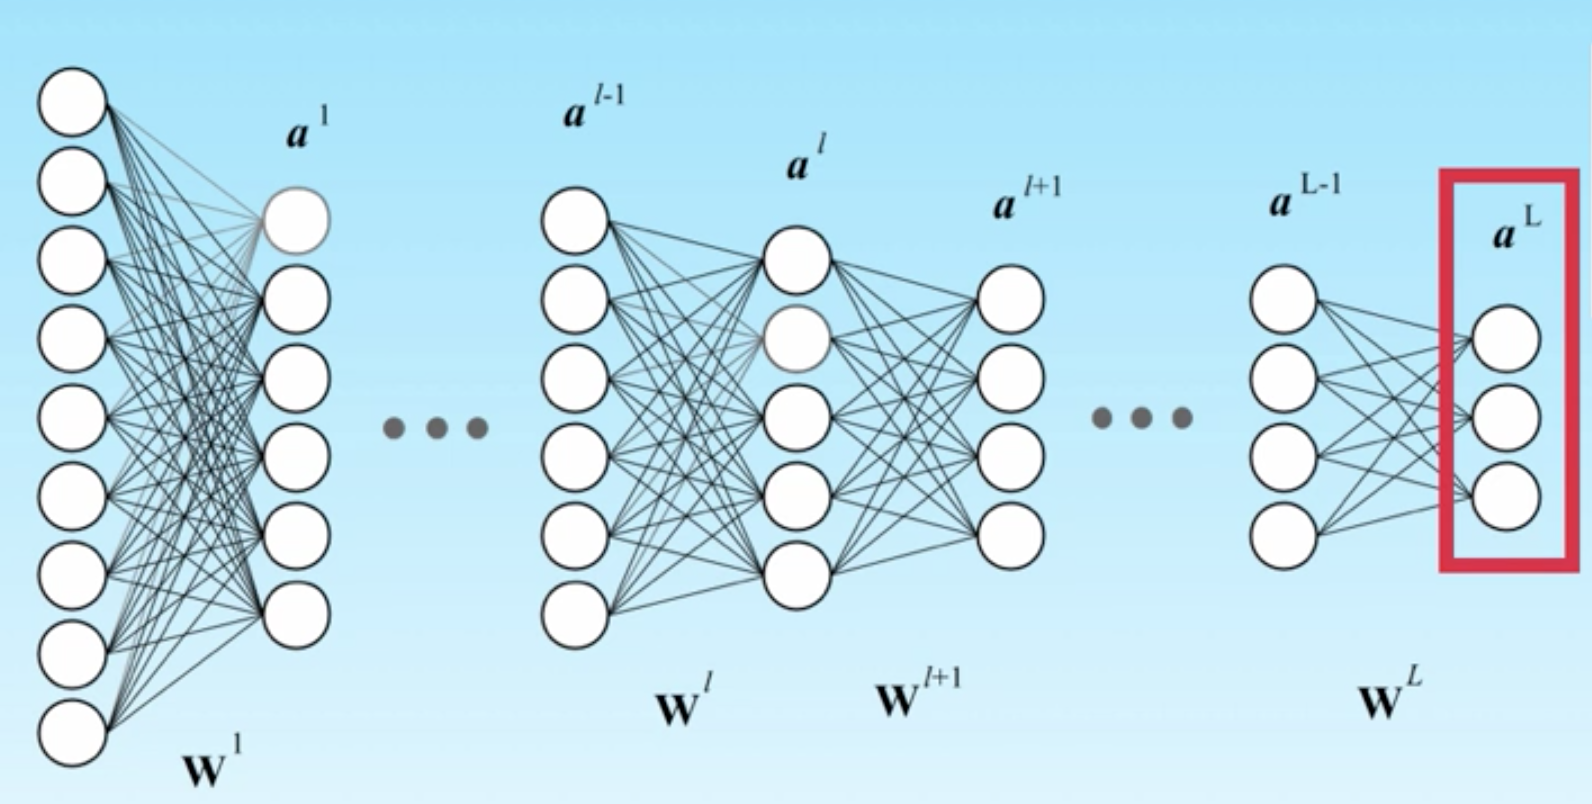
\includegraphics[width=10cm,clip]{nn.png}
	\end{center}
	\caption{This is an illustration of a deep neural network with $p=9$ input features.}\label{fig:1}
\end{figure}
Each layer $l$ is associated with a weight matrix $W^l$, which is $(m\times k)$ with $m$ the number of nodes on the $(l-1)-$th layer and $k$ the number of nodes on the current layer. For example, 
\begin{align}
W^1=\begin{bmatrix} 
W_{11}^1 & \cdots & W_{16}^1 \\
\vdots & \ddots & \vdots\\
W_{91}^1 & \cdots & W_{96}^1
\end{bmatrix}.
\end{align}
The feature matrix $X_{(100\times 9)}$ enters into this neural network and is first multiplied by $W^1_{(9\times 6)}$. Upon adding a bias $b^1_{(6\times 1)}$, we transform the original input into a signal which can be used by the first layer of neurons. In general, the input of layer $l$, which has $k$ nodes, can be written as:
\begin{align}
o^{l-1}_{N\times m}W^l_{(m\times k)} + \boldsymbol{1}_{(N\times 1)}\otimes(b^l_{(k\times 1)})^T
\end{align}
where $o^{l-1}_{N\times m}$ is the output of the previous layer $l-1$ which has $m$ nodes. The component-wise activation function at layer $l$ then transforms the input into an output:
\begin{align}
o^{l}_{N\times k} = \sigma\left( o^{l-1}_{N\times m}W^l_{(m\times k)} + \boldsymbol{1}_{(N\times 1)}\otimes(b^l_{(k\times 1)})^T \right)
\end{align}
At the final layer $L$, the output is $o^L$. Usually, $o^L$ represents the estimated choice probability for each class, and we need to choose the class with the largest estimated probability as our prediction.

\section{Cross-entropy Loss}
After we get our predicions, we want to construct a loss function, which is typically the so-called ``cross-entropy loss'' or negative log-likelihood.

As discussed above, the neural network estimates choice probabilities for each class $c\in\mathcal{J}\equiv\{1,\dots,J\}$:  
\begin{align}
f(\boldsymbol{x})_c = p\left(y=c\vert \boldsymbol{x},\boldsymbol{\theta}\right)
\end{align}
For each datapoint, the likelihood is given by
\begin{align}
 \prod_{c\in\mathcal{J}}p\left(y=c\vert \boldsymbol{x},\boldsymbol{\theta}\right)^{1_{ \{y=c\} }}.
\end{align}
So the negative log-likelihood for one particular data point is 
\begin{align}
l(y\vert \boldsymbol{x},\boldsymbol{\theta}) = -\sum_{c\in\mathcal{J}} 1_{ \{y=c\} } \log p\left(y=c\vert \boldsymbol{x},\boldsymbol{\theta}\right).
\end{align}
Recall that $o^L$ is $(N\times J)$, which gives our predictions of all $N$ individuals. We need the likelihood function for the entire sample. It is not hard to observe that the negative log-likelihood for $N$ individuals under $i.i.d.$ assumption is given by 
\begin{align}
\mathcal{L}(y\vert \boldsymbol{x},\boldsymbol{\theta}) = -\frac{1}{N}\sum_{i=1}^{N}\sum_{c\in\mathcal{J}} 1_{ \{y_i=c\} } \log p\left(y_i=c\vert \boldsymbol{x}_i,\boldsymbol{\theta}\right).
\end{align}
where the scaling factor $1/N$ is added on purpose. In particular, in the binary case where $y_i\in\{0,1\}$, the cross-entropy loss for \textit{each iteration} is
\begin{tcolorbox}
\begin{align}
\mathcal{L}(y\vert \boldsymbol{x},\boldsymbol{\theta}^{(k)}) = -\frac{1}{N}\sum_{i=1}^{N} y_i\log \hat{y}_i^{(k)} + (1-y_i)\log (1-\hat{y}_i^{(k)}).
\end{align}
\end{tcolorbox}
The last line is true because from numeric optimization point of view, for a given iteration, the set of parameters $\boldsymbol{\theta}^{(k)}$ is given, and the neural network will generate exactly $\hat{y}_i^{(k)}=p\left(y_i=1\vert \boldsymbol{x}_i,\boldsymbol{\theta}^{(k)}\right)$ and $1-\hat{y}_i^{(k)}=p\left(y_i=0\vert \boldsymbol{x}_i,\boldsymbol{\theta}^{(k)}\right)$.

Why will the neural network generate exactly the choice probabilities? This comes from multinomial logistic model which we do not discuss in detail here. Recall the softmax activation function: $\sigma:\mathbb{R}^J\to[0,1]^J$
\begin{align}
\sigma(\boldsymbol{z})_j = \frac{e^{z_j}}{\sum_{k=1}^{J}e^{z_k}} \text{, for }j=1,\dots,J.
\end{align}
In artificial neural network, 
\begin{align}
p(y_i=c\vert\boldsymbol{x}_i,\boldsymbol{\theta}) = \frac{e^{\boldsymbol{x}_i^T\boldsymbol{w}_c}}{\sum_{k=1}^{J}e^{\boldsymbol{x}_i^T\boldsymbol{w}_k}} \text{, for }c=1,\dots,J.
\end{align}
Note that in the last layer, the weight matrix $W^L=[\boldsymbol{w}_1,\dots,\boldsymbol{w}_J]$.

\section{Backpropagation}
Suppose at each layer, $z$ is used to denote the input and $o$ is used to denote the output, and let $\delta^l\equiv\frac{\partial \mathcal{L}}{\partial z^l}$. Then, at the last layer $L$, we have:
\begin{align}
\underset{(J\times N)}{\delta^L} =\underset{(J\times N)}{ \bigtriangledown_{o^L}\mathcal{L}}\odot \underset{(J\times N)}{\sigma'(z^L)}
\end{align}
Note that if the last layer has $J$ nodes (which means we have $J$ classes), then both $\Delta_{o^L}\mathcal{L}$ and $\sigma'(z^L)$ are $(J\times N)$ matrices. The $\odot$ is the component wise Hadamard product.

In an inner layer $l$, we have
\begin{align}
\underset{(m\times N)}{\delta^l } = \underset{(m\times k)}{\left(W^{l+1}\right)} \underset{(k\times N)}{\delta^{l+1}}  \odot \underset{(m\times N)}{\sigma'(z^l)}
\end{align}
where we assume there are $m$ nodes in the $l-$th layer and $k$ nodes in the $(l+1)-$th layer.

Finally, to update weights and biases, we calculate
\begin{align}
 \underset{(m\times q)}{\frac{\partial \mathcal{L}}{\partial W^l}} =  \sum_{i=1}^{N} \frac{\partial \mathcal{L}}{\partial z^l_i} \left(\frac{\partial z_i^l}{\partial W^l}\right)^T= \sum_{i=1}^{N} \delta^l_{(\cdot , i)} o^l_{(i,\cdot)} = \underset{(m\times N)}{\delta^l } \underset{(N\times q)}{o^{l-1}}\\
 \underset{(m\times 1)}{\frac{\partial \mathcal{L}}{\partial b^l}} = \sum_{i=1}^{N} \left(\frac{\partial z_i^l}{\partial b^l}\right)\frac{\partial \mathcal{L}}{\partial z^l_i} =  \sum_{i=1}^{N} I_{m\times m}\delta^l_{(\cdot , i)}= \underset{(m\times N)}{\delta^l }\boldsymbol{1}_{N\times 1}
\end{align}
where $q$ is the number of nodes in the $(l-1)-$th layer. This calculation follows from \textit{the chain rule for tensors} (see (6.47) on page 207 in \cite{goodfellow2016deep}).


\subsection{Algorithm}
\textit{step 1)} Forward propagation: get all $o^l$ and $\hat{y}_i$.
~\\
\textit{step 2)} Error in the last layer: $\underset{(J\times N)}{\delta^L} =\underset{(J\times N)}{ \bigtriangledown_{o^L}\mathcal{L}}\odot \underset{(J\times N)}{\sigma'(z^L)}$.
~\\
\textit{step 3)} Backward propagation: calculate $\underset{(m\times N)}{\delta^l } = \underset{(m\times k)}{\left(W^{l+1}\right)} \underset{(k\times N)}{\delta^{l+1}}  \odot \underset{(m\times N)}{\sigma'(z^l)}$
~\\
\textit{step 4)} Derivatives of cost with respect to weight and bias:  $\underset{(m\times q)}{\frac{\partial \mathcal{L}}{\partial W^l}} =  \underset{(m\times N)}{\delta^l } \underset{(N\times q)}{o^{l-1}}\text{, and } \underset{(m\times 1)}{\frac{\partial \mathcal{L}}{\partial b^l}} = \underset{(m\times N)}{\delta^l }\boldsymbol{1}_{N\times 1}$.
~\\
\textit{step 5)} Update weight and bias: $w\to w-\alpha \left(\frac{\partial \mathcal{L}}{\partial W^l}\right)^T$, and $b\to b-\alpha\left(\frac{\partial \mathcal{L}}{\partial b^l}\right)^T$.



\clearpage
\bibliographystyle{chicago}
\bibliography{backprop.bib}


\end{document}